\subsection{Модель сверхширокоугольного объектива}

Сверхширокоугольные объективы имеют в своей основе сложную систему линз, схема которой представлена на рисунке \ref{pic:fyscheme}. 
Особенности этой системы позволяют достигать существенного угла обзора, но также являются причиной аберрации и характерных искажений 
изображения. 

\begin{figure}[H]
    \begin{center}
        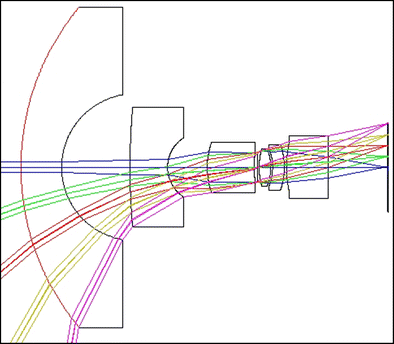
\includegraphics[scale=0.5]{pics/fisheye_scheme.png}                                                                                            %TODO: перерисовать схему?
        \caption{Системы кругового обзора}
        \label{pic:fyscheme}
    \end{center}
\end{figure}
    
Перед использованием снимков с подобных камер необходимо избавиться от искажений. Для осуществления этого необходима модель камеры - 
набор уравнений, который позволяет найти проекцию точки в мировых координатах ${X_w, Y_w, Z_w}$ на точку в плоскости изображения ${u, v}$ и наоборот. 
Перспективная проекция, которая обычно используется для описания камер, не способна спроецировать широкоугольный снимок на кадр конечного размера. Поэтому при производстве
 fisheye-объективов опираются на другие виды проекций \ref{}. Но реальные линзы не всегда в точности следуют заданным моделям, по этой 
 причине для моделирования подобных искажений принято использовать многочлен вида

 \begin{equation}	% TODO: переписать уравнение 
	\begin{split}
        \delta r= k_1 r^3 + k_2 r^5 + k_3 r^7 + ... + k_n r^{n+2}
        \label{eqn:fisheye_distortion}
    \end{split}
\end{equation}

где $k_i$ - коэффициенты, описывающие внутренние параметры камеры. 

В настоящий момент есть несколько распространённых моделей, аппроксимирующих реальные искажения подобных объективов. Модель Канналы и 
Брандта \cite{opencv_model} реализована в OpenCV и описывает радиальные искажения через угол падения луча света на линзу, а не расстояние  
от центра изображения до места падения, как это делалось в более ранних моделях. Авторы посчитали, что для описания типичных искажений достаточно 
пяти членов полинома. Таким образом, указанную модель можно записать следующими уравнениями:

\begin{equation}	
        \theta = \arctan(\frac{r}{f}),
        \label{eqn:kannala_theta}
\end{equation}

\begin{equation}	
    \delta r = k_1\theta + k_2\theta^3 + k_3\theta^5 + k_4\theta^7 + k_5\theta^9,
    \label{eqn:kannala_r}
\end{equation}

\begin{equation}	
    \begin{pmatrix}u\\v\end{pmatrix} = \delta r(\theta)\begin{pmatrix}cos(\phi)\\sin(\phi)\end{pmatrix},
    %\delta r = k_1\theta + k_2\theta^3 + k_3\theta^5 + k_4\theta^7 + ... + k_n\theta^{n+1}
    \label{eqn:kannala_uv}
\end{equation}
где \theta - угол падения луча, определяемый выбранным типом проекции; \phi - угол между горизонтом 
и проекцией падающего луча на плоскость изображения; $r$ - расстояние от спроектированной точки до центра
изображения; $f$ - фокусное расстояние.

Также часто можно встретить модель Скарамуззы \cite{scaramuzza}, которая легла в основу Matlab Omnidirectional 
Camera Calibration Toolbox. Она связывает точки на изображении с соответствующей им точкой в координатах камеры 
следующим образом
\begin{equation}	
    \begin{pmatrix}X_c\\Y_c\\Z_c\end{pmatrix} = \lambda \begin{pmatrix}u\\v\\a_0 + a_2 r^2 + a_3 r^3 + a_4 r^4\end{pmatrix},
    %\delta r = k_1\theta + k_2\theta^3 + k_3\theta^5 + k_4\theta^7 + ... + k_n\theta^{n+1}
    \label{eqn:scaramuzza}
\end{equation}
где $a_0 ... a_4$ - коэффициенты, описывающие внутренние параметры камеры; \lambda - размерный коэффициент.
% TODO: дописать



\subsection{Обзор существующих систем стереозрения, использующих сверхширокоугольные изображения}

Исследователи предложили несколько реализаций стереозрения, опирающихся на снимки со сверхширокоугольных 
объективов. 
Есть классические компланарные методы ... работают только в центральной области. 

Есть неиросетевые методы ...

Были предложены копланарные методы, но до реализации не дошло ...
 